% Options for packages loaded elsewhere
\PassOptionsToPackage{unicode}{hyperref}
\PassOptionsToPackage{hyphens}{url}
\PassOptionsToPackage{dvipsnames,svgnames,x11names}{xcolor}
%
\documentclass[
]{article}
\title{Compulsory Exercise 1}
\usepackage{etoolbox}
\makeatletter
\providecommand{\subtitle}[1]{% add subtitle to \maketitle
  \apptocmd{\@title}{\par {\large #1 \par}}{}{}
}
\makeatother
\subtitle{TMA4268 Statistical Learning V2022}
\author{Emma Skarstein, Daesoo Lee, Stefanie Muff, Department of
Mathematical Sciences, NTNU}
\date{Hand out date: February 7, 2022}

\usepackage{amsmath,amssymb}
\usepackage{lmodern}
\usepackage{iftex}
\ifPDFTeX
  \usepackage[T1]{fontenc}
  \usepackage[utf8]{inputenc}
  \usepackage{textcomp} % provide euro and other symbols
\else % if luatex or xetex
  \usepackage{unicode-math}
  \defaultfontfeatures{Scale=MatchLowercase}
  \defaultfontfeatures[\rmfamily]{Ligatures=TeX,Scale=1}
\fi
% Use upquote if available, for straight quotes in verbatim environments
\IfFileExists{upquote.sty}{\usepackage{upquote}}{}
\IfFileExists{microtype.sty}{% use microtype if available
  \usepackage[]{microtype}
  \UseMicrotypeSet[protrusion]{basicmath} % disable protrusion for tt fonts
}{}
\makeatletter
\@ifundefined{KOMAClassName}{% if non-KOMA class
  \IfFileExists{parskip.sty}{%
    \usepackage{parskip}
  }{% else
    \setlength{\parindent}{0pt}
    \setlength{\parskip}{6pt plus 2pt minus 1pt}}
}{% if KOMA class
  \KOMAoptions{parskip=half}}
\makeatother
\usepackage{xcolor}
\IfFileExists{xurl.sty}{\usepackage{xurl}}{} % add URL line breaks if available
\IfFileExists{bookmark.sty}{\usepackage{bookmark}}{\usepackage{hyperref}}
\hypersetup{
  pdftitle={Compulsory Exercise 1},
  pdfauthor={Emma Skarstein, Daesoo Lee, Stefanie Muff, Department of Mathematical Sciences, NTNU},
  colorlinks=true,
  linkcolor={Maroon},
  filecolor={Maroon},
  citecolor={Blue},
  urlcolor={blue},
  pdfcreator={LaTeX via pandoc}}
\urlstyle{same} % disable monospaced font for URLs
\usepackage[margin=1in]{geometry}
\usepackage{color}
\usepackage{fancyvrb}
\newcommand{\VerbBar}{|}
\newcommand{\VERB}{\Verb[commandchars=\\\{\}]}
\DefineVerbatimEnvironment{Highlighting}{Verbatim}{commandchars=\\\{\}}
% Add ',fontsize=\small' for more characters per line
\usepackage{framed}
\definecolor{shadecolor}{RGB}{248,248,248}
\newenvironment{Shaded}{\begin{snugshade}}{\end{snugshade}}
\newcommand{\AlertTok}[1]{\textcolor[rgb]{0.94,0.16,0.16}{#1}}
\newcommand{\AnnotationTok}[1]{\textcolor[rgb]{0.56,0.35,0.01}{\textbf{\textit{#1}}}}
\newcommand{\AttributeTok}[1]{\textcolor[rgb]{0.77,0.63,0.00}{#1}}
\newcommand{\BaseNTok}[1]{\textcolor[rgb]{0.00,0.00,0.81}{#1}}
\newcommand{\BuiltInTok}[1]{#1}
\newcommand{\CharTok}[1]{\textcolor[rgb]{0.31,0.60,0.02}{#1}}
\newcommand{\CommentTok}[1]{\textcolor[rgb]{0.56,0.35,0.01}{\textit{#1}}}
\newcommand{\CommentVarTok}[1]{\textcolor[rgb]{0.56,0.35,0.01}{\textbf{\textit{#1}}}}
\newcommand{\ConstantTok}[1]{\textcolor[rgb]{0.00,0.00,0.00}{#1}}
\newcommand{\ControlFlowTok}[1]{\textcolor[rgb]{0.13,0.29,0.53}{\textbf{#1}}}
\newcommand{\DataTypeTok}[1]{\textcolor[rgb]{0.13,0.29,0.53}{#1}}
\newcommand{\DecValTok}[1]{\textcolor[rgb]{0.00,0.00,0.81}{#1}}
\newcommand{\DocumentationTok}[1]{\textcolor[rgb]{0.56,0.35,0.01}{\textbf{\textit{#1}}}}
\newcommand{\ErrorTok}[1]{\textcolor[rgb]{0.64,0.00,0.00}{\textbf{#1}}}
\newcommand{\ExtensionTok}[1]{#1}
\newcommand{\FloatTok}[1]{\textcolor[rgb]{0.00,0.00,0.81}{#1}}
\newcommand{\FunctionTok}[1]{\textcolor[rgb]{0.00,0.00,0.00}{#1}}
\newcommand{\ImportTok}[1]{#1}
\newcommand{\InformationTok}[1]{\textcolor[rgb]{0.56,0.35,0.01}{\textbf{\textit{#1}}}}
\newcommand{\KeywordTok}[1]{\textcolor[rgb]{0.13,0.29,0.53}{\textbf{#1}}}
\newcommand{\NormalTok}[1]{#1}
\newcommand{\OperatorTok}[1]{\textcolor[rgb]{0.81,0.36,0.00}{\textbf{#1}}}
\newcommand{\OtherTok}[1]{\textcolor[rgb]{0.56,0.35,0.01}{#1}}
\newcommand{\PreprocessorTok}[1]{\textcolor[rgb]{0.56,0.35,0.01}{\textit{#1}}}
\newcommand{\RegionMarkerTok}[1]{#1}
\newcommand{\SpecialCharTok}[1]{\textcolor[rgb]{0.00,0.00,0.00}{#1}}
\newcommand{\SpecialStringTok}[1]{\textcolor[rgb]{0.31,0.60,0.02}{#1}}
\newcommand{\StringTok}[1]{\textcolor[rgb]{0.31,0.60,0.02}{#1}}
\newcommand{\VariableTok}[1]{\textcolor[rgb]{0.00,0.00,0.00}{#1}}
\newcommand{\VerbatimStringTok}[1]{\textcolor[rgb]{0.31,0.60,0.02}{#1}}
\newcommand{\WarningTok}[1]{\textcolor[rgb]{0.56,0.35,0.01}{\textbf{\textit{#1}}}}
\usepackage{graphicx}
\makeatletter
\def\maxwidth{\ifdim\Gin@nat@width>\linewidth\linewidth\else\Gin@nat@width\fi}
\def\maxheight{\ifdim\Gin@nat@height>\textheight\textheight\else\Gin@nat@height\fi}
\makeatother
% Scale images if necessary, so that they will not overflow the page
% margins by default, and it is still possible to overwrite the defaults
% using explicit options in \includegraphics[width, height, ...]{}
\setkeys{Gin}{width=\maxwidth,height=\maxheight,keepaspectratio}
% Set default figure placement to htbp
\makeatletter
\def\fps@figure{htbp}
\makeatother
\setlength{\emergencystretch}{3em} % prevent overfull lines
\providecommand{\tightlist}{%
  \setlength{\itemsep}{0pt}\setlength{\parskip}{0pt}}
\setcounter{secnumdepth}{-\maxdimen} % remove section numbering
\usepackage{amsmath}
\ifLuaTeX
  \usepackage{selnolig}  % disable illegal ligatures
\fi

\begin{document}
\maketitle

\begin{center}\rule{0.5\linewidth}{0.5pt}\end{center}

\textbf{The submission deadline is: Monday February 21, 23:59h using
Blackboard}

\hypertarget{introduction}{%
\section{Introduction}\label{introduction}}

Maximal score is 40 points. Your score will make up 10\% points of your
final grade.

\hypertarget{supervision}{%
\subsection{Supervision}\label{supervision}}

We will use the times where we would have lectures and exercises for
supervision (4 \(\times\) 2 hours). We will announce the exact
implementation with physical and online supervision as soon as we know.

Supervision hours:

\begin{itemize}
\tightlist
\item
  Monday, February 14, 08:15-10:00 and 14.15-16.00
\item
  Wednesday, February 16, 14.15-16.00
\item
  Thursday February 17, 08.15-10.00
\end{itemize}

Remember that there is also the Mattelab forum, and we strongly
encourage you to use it for your questions outside the supervision hours
-- this ensures that all other students benefit from the answers (try to
avoid emailing the course staff).

\hypertarget{practical-issues-please-read-carefully}{%
\subsection{Practical issues (Please read
carefully)}\label{practical-issues-please-read-carefully}}

\begin{itemize}
\tightlist
\item
  Group size is 2 or 3 - join a group (self enroll) before handing in on
  Blackboard. We prefer that you do not work alone.
\item
  Please organize yourself via the Mattelab discussion forum
  (\url{https://mattelab2022v.math.ntnu.no/c/tma4268/9}) to find a
  group. Once you formed a group, log into Blackboard and add yourself
  to the same group there.
\item
  If you did not find a group even when using Mattelab, you can email
  Stefanie
  (\href{mailto:stefanie.muff@ntnu.no}{\nolinkurl{stefanie.muff@ntnu.no}})
  and I will try to match you with others that are alone (please use
  this really only if you have already tried to find a group).
\item
  Remember to write your names and group number on top of your
  submission file!
\item
  The exercise should be handed in as \textbf{one R Markdown file and a
  pdf-compiled version} of the R Markdown file (if you are not able to
  produce a pdf-file directly please make an html-file, open it in your
  browser and save as pdf - no, not landscape - but portrait please). We
  will read the pdf-file and use the Rmd file in case we need to check
  details in your submission.
\item
  You may want to work through the R Mardown bonus part in the R course
  (\url{https://digit.ntnu.no/courses/course-v1:NTNU+IMF001+2020/about})
\item
  In the R-chunks please use both \texttt{echo=TRUE} and
  \texttt{eval=TRUE} to make it simpler for us to read and grade.
\item
  Please do not include all the text from this file (that you are
  reading now) - we want your R code, plots and written solutions - use
  the template from the course page
  (\url{https://wiki.math.ntnu.no/tma4268/2022v/subpage6}).
\item
  Please \textbf{not more than 12 pages} in your pdf-file! (This is a
  request, not a requirement.)
\item
  Please save us time and \textbf{do not submit word or zip}, and do not
  submit only the Rmd. This only results in extra work for us!
\end{itemize}

\hypertarget{r-packages}{%
\subsection{R packages}\label{r-packages}}

You need to install the following packages in R to run the code in this
file. It is of course also possible to use more or different packages.

\begin{Shaded}
\begin{Highlighting}[]
\FunctionTok{install.packages}\NormalTok{(}\StringTok{"knitr"}\NormalTok{) }\CommentTok{\#probably already installed}
\FunctionTok{install.packages}\NormalTok{(}\StringTok{"rmarkdown"}\NormalTok{) }\CommentTok{\#probably already installed}
\FunctionTok{install.packages}\NormalTok{(}\StringTok{"ggplot2"}\NormalTok{) }\CommentTok{\#plotting with ggplot}
\FunctionTok{install.packages}\NormalTok{(}\StringTok{"palmerpenguins"}\NormalTok{)}
\FunctionTok{install.packages}\NormalTok{(}\StringTok{"ggfortify"}\NormalTok{) }\CommentTok{\# For model checking}
\FunctionTok{install.packages}\NormalTok{(}\StringTok{"MASS"}\NormalTok{)}
\FunctionTok{install.packages}\NormalTok{(}\StringTok{"class"}\NormalTok{)}
\FunctionTok{install.packages}\NormalTok{(}\StringTok{"pROC"}\NormalTok{)}
\FunctionTok{install.packages}\NormalTok{(}\StringTok{"plotROC"}\NormalTok{)}
\FunctionTok{install.packages}\NormalTok{(}\StringTok{"boot"}\NormalTok{)}
\end{Highlighting}
\end{Shaded}

\hypertarget{multiplesingle-choice-problems}{%
\subsection{Multiple/single choice
problems}\label{multiplesingle-choice-problems}}

There will be a few \emph{multiple and single choice questions}. This is
how these will be graded:

\begin{itemize}
\item
  \textbf{Multiple choice questions (2P)}: There are four choices, and
  each of them can be TRUE or FALSE. If you make one mistake (either
  wrongly mark an option as TRUE/FALSE) you get 1P, if you have two or
  more mistakes, you get 0P. Your answer should be given as a list of
  answers, like TRUE, TRUE, FALSE, FALSE, for example.
\item
  \textbf{Single choice questions (1P)}: There are several choices, and
  only \emph{one} of the alternatives is the correct one. You will
  receive 1P if you choose the correct alternative and 0P if you choose
  wrong. Only say which option is true (for example (ii)).
\end{itemize}

\hypertarget{problem-1-8p}{%
\section{Problem 1 (8P)}\label{problem-1-8p}}

We have a univariate continuous random variable \(Y\) and a covariate
\(x\). Further, we have observed a training set of independent
observation pairs \(\{x_i, y_i\}\) for \(i=1,\ldots,n\). Assume a
regression model \[Y_i  = f(x_i) + \varepsilon_i \ ,\] where \(f\) is
the true regression function, and \(\varepsilon_i\) is an unobserved
random variable with mean zero and constant variance \(\sigma^2\) (not
dependent on the covariate). Using the training set we can find an
estimate of the regression function \(f\), and we denote this by
\(\hat{f}\). We want to use \(\hat{f}\) to make a prediction for a new
observation (not dependent on the observations in the training set) at a
covariate value \(x_0\). The predicted response value is then
\(\hat{f}(x_0)\). We are interested in the error associated with this
prediction.

\hypertarget{a-2p}{%
\subsection{a) (2P)}\label{a-2p}}

Derive the decomposition of the expected test MSE,
\(E[y_0 - \hat{f}(x_0)]^2\), into three terms (bias, variance, and
irreducible error).

\hypertarget{b-1p}{%
\subsection{b) (1P)}\label{b-1p}}

Explain with words how we can interpret the three terms.

\hypertarget{c-2p---multiple-choice}{%
\subsection{c) (2P) - Multiple choice}\label{c-2p---multiple-choice}}

Figure 1 shows the squared bias, variance, irreducible error and total
error for increasing values of \(K\) in KNN regression. Which of the
following statements are true and which are false? Say for \emph{each}
of them if it is true or false.

\begin{enumerate}
\def\labelenumi{(\roman{enumi})}
\tightlist
\item
  Decreased \(K\) corresponds to increased flexibility of the model.
\item
  The variance increases with increased value of \(K\).
\item
  The blue line corresponds to the irreducible error.
\item
  The squared bias decreases with increased value of \(K\).
\end{enumerate}

\begin{figure}
\centering
\includegraphics[width=0.5\textwidth,height=\textheight]{BiasVarTradeOff.png}
\caption{Squared bias, variance, irreducible error and total error for
increasing values of \(K\) in KNN}
\end{figure}

\hypertarget{d-2p-multiple-choice}{%
\subsection{d) (2P) Multiple choice}\label{d-2p-multiple-choice}}

Which of the following statements are true and which are false? Say for
\emph{each} of them if it is true or false.

\begin{enumerate}
\def\labelenumi{(\roman{enumi})}
\tightlist
\item
  If the relationship between the predictors and response is highly
  non-linear, a flexible method will generally perform better than an
  inflexible method.
\item
  If the number of predictors \(p\) is extremely large and the number of
  observations \(n\) is small, a flexible method will generally perform
  better than an inflexible method.
\item
  In KNN classification, it is important to use the test set to select
  the value \(K\), and not the training set, to avoid overfitting.
\item
  In a linear regression setting, adding more covariates will reduce the
  variance of the predictor function.
\end{enumerate}

\hypertarget{e-1p-single-choice}{%
\subsection{e) (1P) Single choice}\label{e-1p-single-choice}}

\(\mathbf{X} = [x_1, x_2, x_3]^T\) is a 3-dimensional random vector with
covariance matrix \[
\boldsymbol{\Sigma} = \begin{bmatrix}
  50 & 33 & 18 \\
  33 & 38 & -10 \\
  18 & -10  & 72
  \end{bmatrix}
\]

The correlation between element \(x_1\) and \(x_2\) of the vector
\(\mathbf{X}\) is:

\begin{enumerate}
\def\labelenumi{(\roman{enumi})}
\tightlist
\item
  0.017
\item
  -0.19
\item
  0.76
\item
  0.66
\item
  0.10
\item
  0.3
\item
  It is not possible to calculate the correlation, because this is not a
  proper covariance matrix.
\end{enumerate}

\hypertarget{problem-2-9p}{%
\section{Problem 2 (9P)}\label{problem-2-9p}}

In the following example, Basil has been given a dataset by his boss.
The dataset consists of observations of Antarctic penguins who live on
the Palmer Archipelago. Basil's boss wonders if he can set up a model to
predict the body mass of a given penguin based on some recorded
characteristics of the penguin, which are specified in advance based on
expert knowledge. However, Basil is a cat, and despite being very
clever, he has only a very rudimentary knowledge of statistical
techniques and data analysis. In the following code and report, Basil
has made a couple of very problematic mistakes.

\begin{center}\rule{0.5\linewidth}{0.5pt}\end{center}

\begin{Shaded}
\begin{Highlighting}[]
\DocumentationTok{\#\#\#\#\#\#\#\#\#\#\#\#\#\# =\^{}.\_.\^{}=  \textasciitilde{}\textasciitilde{}\textasciitilde{}BASIL\textquotesingle{}S CODE\textasciitilde{}\textasciitilde{}\textasciitilde{}  =\^{}.\_.\^{}= \#\#\#\#\#\#\#\#\#\#\#\#\#\# }
\CommentTok{\#install.packages("palmerpenguins")  \# Run if you haven\textquotesingle{}t installed this before.}
\FunctionTok{library}\NormalTok{(palmerpenguins) }\CommentTok{\# Contains the data set "penguins".}
\FunctionTok{data}\NormalTok{(penguins)}

\CommentTok{\# Remove island, and year variable, as we won\textquotesingle{}t use those.}
\NormalTok{Penguins }\OtherTok{\textless{}{-}} \FunctionTok{subset}\NormalTok{(penguins, }\AttributeTok{select =} \SpecialCharTok{{-}}\FunctionTok{c}\NormalTok{(island, year))}

\CommentTok{\# Fit the model as specified in advance based on expert knowledge:}
\NormalTok{penguin.model }\OtherTok{\textless{}{-}} \FunctionTok{lm}\NormalTok{(body\_mass\_g }\SpecialCharTok{\textasciitilde{}}\NormalTok{ flipper\_length\_mm }\SpecialCharTok{+}\NormalTok{ sex }\SpecialCharTok{+}\NormalTok{ bill\_depth\_mm}\SpecialCharTok{*}\NormalTok{species, }
                    \AttributeTok{data =}\NormalTok{ Penguins)}

\CommentTok{\# Look at the model coefficients}
\FunctionTok{summary}\NormalTok{(penguin.model)}\SpecialCharTok{$}\NormalTok{coefficients}
\end{Highlighting}
\end{Shaded}

\begin{verbatim}
##                                   Estimate Std. Error   t value     Pr(>|t|)
## (Intercept)                    -1336.58287 646.922248 -2.066064 3.961450e-02
## flipper_length_mm                 17.37877   2.910449  5.971165 6.172012e-09
## sexmale                          432.90151  44.633685  9.698987 1.059323e-19
## bill_depth_mm                     82.98484  22.324227  3.717255 2.370966e-04
## speciesChinstrap                1460.14721 680.389708  2.146045 3.260954e-02
## speciesGentoo                    644.88114 542.573989  1.188559 2.354811e-01
## bill_depth_mm:speciesChinstrap   -83.53310  37.009147 -2.257093 2.466587e-02
## bill_depth_mm:speciesGentoo       36.17178  34.481962  1.049006 2.949549e-01
\end{verbatim}

\begin{Shaded}
\begin{Highlighting}[]
\CommentTok{\# Fit final model without sex}
\NormalTok{final.model }\OtherTok{\textless{}{-}} \FunctionTok{lm}\NormalTok{(body\_mass\_g }\SpecialCharTok{\textasciitilde{}}\NormalTok{ flipper\_length\_mm }\SpecialCharTok{+}\NormalTok{ bill\_depth\_mm}\SpecialCharTok{*}\NormalTok{species, }
                  \AttributeTok{data =}\NormalTok{ Penguins)}

\FunctionTok{summary}\NormalTok{(final.model)}
\end{Highlighting}
\end{Shaded}

\begin{verbatim}
## 
## Call:
## lm(formula = body_mass_g ~ flipper_length_mm + bill_depth_mm * 
##     species, data = Penguins)
## 
## Residuals:
##     Min      1Q  Median      3Q     Max 
## -895.42 -226.28  -24.56  207.65 1074.66 
## 
## Coefficients:
##                                 Estimate Std. Error t value Pr(>|t|)    
## (Intercept)                    -4213.176    647.731  -6.505 2.84e-10 ***
## flipper_length_mm                 24.621      3.173   7.760 1.04e-13 ***
## bill_depth_mm                    176.443     22.580   7.814 7.22e-14 ***
## speciesChinstrap                1008.380    771.358   1.307   0.1920    
## speciesGentoo                    129.453    608.383   0.213   0.8316    
## bill_depth_mm:speciesChinstrap   -61.538     41.978  -1.466   0.1436    
## bill_depth_mm:speciesGentoo       78.026     38.545   2.024   0.0437 *  
## ---
## Signif. codes:  0 '***' 0.001 '**' 0.01 '*' 0.05 '.' 0.1 ' ' 1
## 
## Residual standard error: 327.3 on 335 degrees of freedom
##   (2 observations deleted due to missingness)
## Multiple R-squared:  0.8364, Adjusted R-squared:  0.8335 
## F-statistic: 285.5 on 6 and 335 DF,  p-value: < 2.2e-16
\end{verbatim}

\begin{quote}
\textbf{\emph{REPORT: PREDICTION OF PENGUIN BODY MASS, by Basil Thecat
:3}}\\
We begin with a linear regression model with body mass as the response,
and flipper length, bill depth, species, and sex as covariates, as well
as an interaction effect between bill depth and species. In this first
model, the sex covariate has the smallest \(p\)-value and is thus
excluded in the final model to avoid overfitting. The final model can be
described depending on the species of the penguin: \[
\begin{aligned}
\hat{y}_{adelie} &= \hat\beta_0 + \hat\beta_{flipper\_length} x_{flipper\_length} +      \hat\beta_{bill\_depth} x_{bill\_depth} \\
\hat{y}_{chinstrap} &= \hat\beta_0 + \hat\beta_{flipper\_length} x_{flipper\_length} + (\hat\beta_{bill\_depth} + \hat\beta_{bill\_depth:chinstrap}) x_{bill\_depth} + \hat\beta_{chinstrap} \\
\hat{y}_{gentoo} &= \hat\beta_0 + \hat\beta_{flipper\_length} x_{flipper\_length} + (\hat\beta_{bill\_depth} + \hat\beta_{bill\_depth:gentoo}) x_{bill\_depth} + \hat\beta_{gentoo} 
\end{aligned}
\] (where \(\hat y_{adelie}\) is the predicted body mass for Adelie
penguins, \(\hat\beta_0\) is the estimated intercept,
\(x_{flipper\_length}\) is the flipper length covariate,
\(\hat\beta_{flipper\_length}\) is the estimated flipper length
coefficient, etc.) Since both of the species coefficients have large
\(p\)-values, we do not reject the null hypothesis that the species
coefficient overall is actually zero. For the interaction effect between
species and bill depth, the Gentoo interaction is significant
\((p<0.05\)), so the interaction term overall is significant. Based on
the coefficient for the dummy variable for the chinstrap penguins being
the largest (\(\hat\beta_{chinstrap} \approx 1008\)), we can tell that
the chinstrap penguins have the largest body mass.
\end{quote}

\hypertarget{a-3p}{%
\subsection{a) (3P)}\label{a-3p}}

Identify three of the mistakes Basil made (there are more than three,
but only report three). List them as bullet points along with brief
explanations of why these are inappropriate modeling choices.

1)Basel have understood the meaning of p-values. He has excluded the sex
covariate as he mentioned that it has the smallest p-value. However, a
small p-value indicates that the sex covariate has significant
importance in determine the body mass of penguins. A F-test should be
conducted before the choice of omitting the sex covariate.\\
2)The body mass of penguins has been described to be dependent on the
species of the penguin. This done despite the fact that species have the
highest p-value in the original model. This is evident by an extremely
high p-value for the species coefficients in the final model which
suggests that there is a high probability for observing the null
hypothesis, where there is no relationship between species and body
mass.A F-test can be conducted to determine if species should be
omitted. 3)Basel concludes that chinstrap penguins have the largest body
mass from the fact that the dummy variable for chinstrap penguins have
the largest value. However he does not consider that the interaction
effect between bill depth and Chinstrap is the only negative term while
the others are positive. The final body mass for chinstraps can
therefore be lower than the other species due to this interaction term.

\hypertarget{b-1p-1}{%
\subsection{b) (1P)}\label{b-1p-1}}

In order to make an improved model, you will need to understand the
data. Create at least one informative plot that helps you explain at
least one of Basil's mistakes and that will justify your modeling
choices in the next step. (Plotting the data may even help you
\emph{discover} Basil's mistakes in the first place.)

\begin{center}\rule{0.5\linewidth}{0.5pt}\end{center}

\begin{Shaded}
\begin{Highlighting}[]
\DocumentationTok{\#\#\#\#\#\#\#\#\#\#\#\#\#\# =\^{}.\_.\^{}=  \textasciitilde{}\textasciitilde{}\textasciitilde{}BASIL\textquotesingle{}S CODE\textasciitilde{}\textasciitilde{}\textasciitilde{}  =\^{}.\_.\^{}= \#\#\#\#\#\#\#\#\#\#\#\#\#\# }
\CommentTok{\#install.packages("palmerpenguins")  \# Run if you haven\textquotesingle{}t installed this before.}
\FunctionTok{library}\NormalTok{(GGally)}

\FunctionTok{library}\NormalTok{(palmerpenguins) }\CommentTok{\# Contains the data set "penguins".}
\FunctionTok{data}\NormalTok{(penguins)}

\CommentTok{\# Remove island, and year variable, as we won\textquotesingle{}t use those.}
\NormalTok{Penguins }\OtherTok{\textless{}{-}} \FunctionTok{subset}\NormalTok{(penguins, }\AttributeTok{select =} \SpecialCharTok{{-}}\FunctionTok{c}\NormalTok{(island, year))}


\FunctionTok{ggpairs}\NormalTok{(Penguins)}
\end{Highlighting}
\end{Shaded}

\begin{center}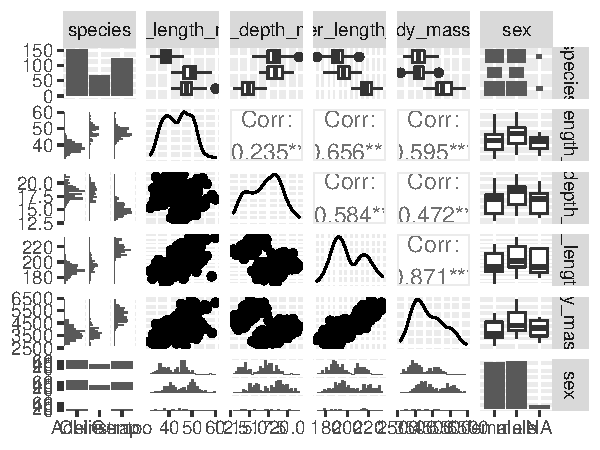
\includegraphics{Compulsory1_files/figure-latex/unnamed-chunk-3-1} \end{center}

\hypertarget{c-5p}{%
\subsection{c) (5P)}\label{c-5p}}

Redo Basil's analysis including code and report, this time doing it
right (4P). Evaluate the fit of the model with at least one graphical
tool (1P).

\hypertarget{problem-3-13p}{%
\section{Problem 3 (13P)}\label{problem-3-13p}}

We will now consider the Palmer penguin dataset again, but this time
looking at classifying the species of the penguins for a given body mass
and flipper length. Since there are three penguin species, for
simplicity we will define the goal to be to classify a penguin as
belonging to the species Adelie or \emph{not} Adelie, giving us a
two-class classification problem instead of three.

The following code modifies the data set for this simplified setting,
converts the variables to numeric (because the \texttt{knn} function
can't handle the \texttt{int} class, and will give an error), and
removes any missing observations. Please remember to use the same seed
when you split the data into training and test set.

\begin{Shaded}
\begin{Highlighting}[]
\FunctionTok{library}\NormalTok{(tidyverse)}
\FunctionTok{library}\NormalTok{(GGally)}
\CommentTok{\# Create a new boolean variable indicating whether or not the penguin is an Adelie penguin}
\NormalTok{Penguins}\SpecialCharTok{$}\NormalTok{adelie }\OtherTok{\textless{}{-}} \FunctionTok{ifelse}\NormalTok{(Penguins}\SpecialCharTok{$}\NormalTok{species }\SpecialCharTok{==} \StringTok{"Adelie"}\NormalTok{, }\DecValTok{1}\NormalTok{, }\DecValTok{0}\NormalTok{)}

\CommentTok{\# Select only relevant variables and remove all rows with missing values in }
\CommentTok{\# body mass, flipper length, sex or species.}
\NormalTok{Penguins\_reduced }\OtherTok{\textless{}{-}}\NormalTok{ Penguins }\SpecialCharTok{\%\textgreater{}\%} 
\NormalTok{  dplyr}\SpecialCharTok{::}\FunctionTok{select}\NormalTok{(body\_mass\_g, flipper\_length\_mm, adelie) }\SpecialCharTok{\%\textgreater{}\%} 
  \FunctionTok{mutate}\NormalTok{(}\AttributeTok{body\_mass\_g =} \FunctionTok{as.numeric}\NormalTok{(body\_mass\_g), }
         \AttributeTok{flipper\_length\_mm =} \FunctionTok{as.numeric}\NormalTok{(flipper\_length\_mm)) }\SpecialCharTok{\%\textgreater{}\%} 
  \FunctionTok{drop\_na}\NormalTok{()}

\FunctionTok{set.seed}\NormalTok{(}\DecValTok{4268}\NormalTok{) }

\CommentTok{\# 70\% of the sample size for training set}
\NormalTok{training\_set\_size }\OtherTok{\textless{}{-}} \FunctionTok{floor}\NormalTok{(}\FloatTok{0.70} \SpecialCharTok{*} \FunctionTok{nrow}\NormalTok{(Penguins\_reduced))}

\NormalTok{train\_ind }\OtherTok{\textless{}{-}} \FunctionTok{sample}\NormalTok{(}\FunctionTok{seq\_len}\NormalTok{(}\FunctionTok{nrow}\NormalTok{(Penguins\_reduced)), }\AttributeTok{size =}\NormalTok{ training\_set\_size)}

\NormalTok{train }\OtherTok{\textless{}{-}}\NormalTok{ Penguins\_reduced[train\_ind, ]}
\NormalTok{test }\OtherTok{\textless{}{-}}\NormalTok{ Penguins\_reduced[}\SpecialCharTok{{-}}\NormalTok{train\_ind, ]}
\end{Highlighting}
\end{Shaded}

\hypertarget{a-5p}{%
\subsection{a) (5P)}\label{a-5p}}

\begin{enumerate}
\def\labelenumi{(\roman{enumi})}
\item
  (1P) Fit a \textbf{logistic regression} model using the training set,
  and perform the classification on the test set, using a 0.5 cutoff.
\item
  (1P) Fit a \textbf{QDA} model using the training set, and perform the
  classification on the test set, using a 0.5 cutoff.
\item
  (1P) Finally, do the same as in (i) and (ii) using \textbf{KNN} with
  \(k = 25\) (use the \texttt{knn} function from the \texttt{class}
  package).
\end{enumerate}

\textbf{R-hints:} In the \texttt{knn()} function set \texttt{prob=T} to
ensure you get the class probabilities that you then need in d):

\begin{Shaded}
\begin{Highlighting}[]
\NormalTok{knnMod }\OtherTok{=} \FunctionTok{knn}\NormalTok{(}\AttributeTok{train =}\NormalTok{ ..., }\AttributeTok{test =}\NormalTok{ ..., }\AttributeTok{cl =}\NormalTok{ ..., }\AttributeTok{k =} \DecValTok{25}\NormalTok{, }\AttributeTok{prob =}\NormalTok{ T)}
\end{Highlighting}
\end{Shaded}

\begin{enumerate}
\def\labelenumi{(\roman{enumi})}
\setcounter{enumi}{3}
\tightlist
\item
  (2P) Calculate the sensitivity and specificity for the three
  predictions performed on the test set in (i) - (iii).
\end{enumerate}

\hypertarget{b-5p}{%
\subsection{b) (5P)}\label{b-5p}}

\begin{enumerate}
\def\labelenumi{(\roman{enumi})}
\tightlist
\item
  Present a plot of the ROC curves and calculate the area under the
  curve (AUC) for each of the classifiers in a) (1P for each model).
\item
  Briefly discuss the ROC curves and the AUC. Which model performs best
  and worst (1P)?
\item
  If the task is to create an interpretable model, which model would you
  choose (1P)?
\end{enumerate}

\textbf{R-hints:}

\begin{itemize}
\tightlist
\item
  To obtain \(P(y=1)\) from the \texttt{knn()} output you have to be
  aware that the respective probabilities
\end{itemize}

\begin{Shaded}
\begin{Highlighting}[]
\FunctionTok{attributes}\NormalTok{(knnMod)}\SpecialCharTok{$}\NormalTok{prob}
\end{Highlighting}
\end{Shaded}

are the success probability for the actual class where the
categorization was made. So if you want to get a vector for \(P(y=1)\),
you have to use \(1-P(y=0)\) for the cases where the categorization was
0:

\begin{Shaded}
\begin{Highlighting}[]
\NormalTok{probKNN }\OtherTok{=}\FunctionTok{ifelse}\NormalTok{(knnMod}\SpecialCharTok{==}\DecValTok{0}\NormalTok{, }\DecValTok{1} \SpecialCharTok{{-}} \FunctionTok{attributes}\NormalTok{(knnMod)}\SpecialCharTok{$}\NormalTok{prob,}\FunctionTok{attributes}\NormalTok{(knnMod)}\SpecialCharTok{$}\NormalTok{prob)}
\end{Highlighting}
\end{Shaded}

\begin{itemize}
\tightlist
\item
  You might find the functions \texttt{roc()} and \texttt{ggroc()} from
  the package \texttt{pROC} useful, but there are many ways to plot ROC
  curves.
\end{itemize}

\hypertarget{c-1p-single-choice}{%
\subsection{c) (1P) Single choice}\label{c-1p-single-choice}}

We are again looking at the logistic regression model that you fitted to
the training data in a).

According to this model, how would the odds that an observed animal is
from the \emph{Adelie} species change if the body mass increases by 1000
g? (the flipper length stays the same)

\begin{enumerate}
\def\labelenumi{\roman{enumi})}
\tightlist
\item
  We add 0.359.
\item
  We multiply it with 0.001.
\item
  We multiply by 1.432.
\item
  We multiply by 0.359.
\item
  We add 1.432.
\item
  We multiply by 1000.
\end{enumerate}

\hypertarget{d-2p}{%
\subsection{d) (2P)}\label{d-2p}}

Plot the full data (including both training nd test set) with the two
covariates as the \(x\)- and \(y\)-axis, and use color and some other
attribute of your choice (e.g.~shape or highlight) to visualize the true
species (adelie/not adelie) as well as the predicted species from the
best model in b) (note that the model should only be fitted with the
training data as in b), but you are showing the data and predictions for
both training and test data in the same plot).

\hypertarget{problem-4-10p}{%
\section{Problem 4 (10P)}\label{problem-4-10p}}

\hypertarget{a-2p---multiple-choice}{%
\subsection{a) (2P) - Multiple choice}\label{a-2p---multiple-choice}}

Which statements about validation set approach, \(k\)-fold
cross-validation (CV) and leave-one-out cross validation (LOOCV) are
true and which are false? Say for \emph{each} of them if it is true or
false.

\begin{enumerate}
\def\labelenumi{(\roman{enumi})}
\tightlist
\item
  The validation set-approach is computationally cheaper than
  \(10\)-fold CV.
\item
  5-fold CV will generally lead to less bias, but more variance than
  LOOCV in the estimated prediction error.
\item
  The validation set-approach is the same as \(2\)-fold CV.
\item
  LOOCV is always the cheapest way to do cross-validation.
\end{enumerate}

\hypertarget{b-2p}{%
\subsection{b) (2P)}\label{b-2p}}

We are now looking at a bootstrap example. Assume you want to fit a
model that predicts the probability for coronary heart disease
(\texttt{chd}) from systolic blood pressure (\texttt{sbp}), sex
(0=female, 1=male) and smoking status (0=no, 1=yes). Load the data in R
as follows

\begin{Shaded}
\begin{Highlighting}[]
\NormalTok{id }\OtherTok{\textless{}{-}} \StringTok{"1chRpybM5cJn4Eow3{-}\_xwDKPKyddL9M2N"} \CommentTok{\# google file ID}
\NormalTok{d.chd }\OtherTok{\textless{}{-}} \FunctionTok{read.csv}\NormalTok{(}\FunctionTok{sprintf}\NormalTok{(}\StringTok{"https://docs.google.com/uc?id=\%s\&export=download"}\NormalTok{, id))}
\end{Highlighting}
\end{Shaded}

and perform a logistic regression with \texttt{chd} as outcome and
\texttt{sbp}, \texttt{sex} and \texttt{smoking} as covariates. What is
the probability of chd for a non-smoking male with a sbp=150 in the
given dataset?

\hypertarget{c-4p}{%
\subsection{c) (4P)}\label{c-4p}}

We now use the bootstrap to estimate the uncertainty of the probability
derived in b). Use \(B=1000\) bootstrap samples and proceed as follows:

\begin{itemize}
\tightlist
\item
  In each iteration, derive and store the estimated probability for
  \texttt{chd}, given \texttt{sbp}=150, \texttt{sex}=male and
  \texttt{smoking}=0 (1P for implementing the bootstrap).
\item
  From the set of estimated probabilities, derive the standard error
  (1P).
\item
  Derive the 95\% quantile interval for the bootstrap samples (that is,
  the interval with limits at 2.5\% and 97.5\%) (1P).
\item
  Interpret what you see. What is the expected probability and what are
  plausible values? (1P)
\end{itemize}

\hypertarget{d-multiple-choice---2p}{%
\subsection{d) Multiple choice - 2P}\label{d-multiple-choice---2p}}

We continue with the same dataset to study some properties of the
bootstrap method. Below we estimated the standard errors of the
regression coefficients in the logistic regression model with
\texttt{sex}, \texttt{sbp} and \texttt{smoking} as predictors using 1000
bootstrap iterations (column \texttt{std.error}). These standard errors
can be compared to those that we obtain by fitting a single logistic
regression model using the \texttt{glm()} function (in Problem 4b). Look
at the R output below and compare the standard errors that we obtain
from the bootstrap with those we get from the \texttt{glm()} function
(note that the \texttt{t1*} to \texttt{t4*} variables are sorted in the
same way as for the \texttt{glm()} output).

\begin{Shaded}
\begin{Highlighting}[]
\FunctionTok{set.seed}\NormalTok{(}\DecValTok{4268}\NormalTok{)}
\FunctionTok{library}\NormalTok{(boot)}
\NormalTok{boot.fn }\OtherTok{\textless{}{-}} \ControlFlowTok{function}\NormalTok{(data,index)\{}
  \FunctionTok{return}\NormalTok{(}\FunctionTok{coefficients}\NormalTok{(}\FunctionTok{glm}\NormalTok{(chd }\SpecialCharTok{\textasciitilde{}}\NormalTok{ sbp }\SpecialCharTok{+}\NormalTok{ sex }\SpecialCharTok{+}\NormalTok{ smoking, }\AttributeTok{family=}\StringTok{"binomial"}\NormalTok{,}\AttributeTok{data=}\NormalTok{data,}\AttributeTok{subset=}\NormalTok{index)))}
\NormalTok{\}}
\FunctionTok{boot}\NormalTok{(d.chd,boot.fn,}\DecValTok{1000}\NormalTok{)}
\end{Highlighting}
\end{Shaded}

\begin{verbatim}
## 
## ORDINARY NONPARAMETRIC BOOTSTRAP
## 
## 
## Call:
## boot(data = d.chd, statistic = boot.fn, R = 1000)
## 
## 
## Bootstrap Statistics :
##        original        bias    std. error
## t1* -6.65883685  0.0142486669  2.54155686
## t2*  0.03877165 -0.0001413491  0.01921332
## t3* -1.34351384 -0.0462122125  0.33868464
## t4*  0.41031080 -0.0220322661  0.33473663
\end{verbatim}

Which of the following statements are true? Say for \emph{each} of them
if it is true or false.

\begin{enumerate}
\def\labelenumi{(\roman{enumi})}
\tightlist
\item
  The bootstrap relies on random sampling the same data without
  replacement.
\item
  The estimated standard errors from the \texttt{glm()} function are
  smaller than those estimated from the bootstrap, which indicates a
  problem with the bootstrap.
\item
  In general, differences between the estimated standard errors from the
  bootstrap and those from \texttt{glm()} may indicate a problem with
  the assumptions taken in logistic regression.
\item
  The \(p\)-values from the \texttt{glm()} output are probably slightly
  too small.
\end{enumerate}

\end{document}
